\chapter{Cơ sở lý thuyết và các công trình liên quan}
\label{ch:related}

Chương này trình bày các cơ sở lý thuyết trực tiếp phục vụ thiết kế ở \cref{ch:method}, gồm attention cửa sổ, mô hình không gian trạng thái chọn lọc, pipeline STAD hai giai đoạn và hàm mất mát cho dữ liệu mất cân bằng; sau đó tổng quan các họ phương pháp liên quan và rút ra khoảng trống nghiên cứu.

\section{Cơ sở lý thuyết}
\label{sec:theory}

\subsection{Self-attention và attention trong cửa sổ}
\label{sec:attention}

Cho chuỗi $T$ token $\mat{X} \in \R^{T \times C}$, self-attention \cite{vaswani2017attention} tính các phép chiếu $\mat{Q} = \mat{X}\mat{W}_Q$, $\mat{K} = \mat{X}\mat{W}_K$, $\mat{V} = \mat{X}\mat{W}_V$ và trả ra
\begin{equation}
\mathrm{Attn}(\mat{X}) = \softmax\!\left(\frac{\mat{Q}\mat{K}^{\top}}{\sqrt{d}} + \mat{M}\right)\mat{V},
\label{eq:attention}
\end{equation}
trong đó $d$ là số chiều mỗi đầu và $\mat{M} \in \{0, -\infty\}^{T \times T}$ là mặt nạ. Với $\mat{M} = \mat{0}$, mọi cặp token được so khớp với chi phí $O(T^2 d)$. Multi-head self-attention (MHSA) chia $C$ kênh thành $h$ đầu, mỗi đầu học một kiểu quan hệ riêng. Khi đặt $M_{ij} = -\infty$ cho mọi $|i - j| > \lfloor W/2 \rfloor$, attention chỉ còn tác dụng trong một \emph{cửa sổ trượt} độ rộng $W$ quanh mỗi token \cite{beltagy2020longformer}; số cặp có ích giảm từ $T^2$ xuống $TW$. Swin Transformer \cite{liu2021swin} và Video Swin \cite{liu2022videoswin} áp dụng ý tưởng cửa sổ trong không gian và thời gian, với các cửa sổ dịch chuyển xen kẽ để thông tin lan truyền qua nhiều tầng.

\subsection{Mô hình không gian trạng thái chọn lọc}
\label{sec:ssm}

Một mô hình không gian trạng thái (SSM) tuyến tính liên tục ánh xạ tín hiệu vào $x(t)$ sang tín hiệu ra $y(t)$ thông qua trạng thái ẩn $\mat{h}(t) \in \R^{N}$:
\begin{equation}
\mat{h}'(t) = \mat{A}\mat{h}(t) + \mat{B}x(t), \qquad y(t) = \mat{C}\mat{h}(t) + Dx(t).
\label{eq:ssm-cont}
\end{equation}
Rời rạc hóa với bước $\Delta$ (zero-order hold) cho dạng hồi quy
\begin{equation}
\begin{gathered}
\mat{h}_t = \bar{\mat{A}}\mat{h}_{t-1} + \bar{\mat{B}}x_t, \qquad y_t = \mat{C}\mat{h}_t + Dx_t,\\
\bar{\mat{A}} = e^{\Delta\mat{A}}, \qquad \bar{\mat{B}} = (\Delta\mat{A})^{-1}(e^{\Delta\mat{A}} - \mat{I})\Delta\mat{B}.
\end{gathered}
\label{eq:ssm-disc}
\end{equation}
S4 \cite{gu2022s4} chỉ ra rằng với $\mat{A}$ có cấu trúc phù hợp, hồi quy này huấn luyện ổn định trên chuỗi hàng nghìn bước, nhưng các tham số $(\Delta, \mat{B}, \mat{C})$ bất biến theo thời gian nên mô hình không thể ``chọn'' giữ hay quên thông tin theo nội dung. Mamba \cite{gu2023mamba} đưa vào \emph{tính chọn lọc}: $\Delta_t$, $\mat{B}_t$ và $\mat{C}_t$ được sinh từ chính $x_t$, trong khi $\mat{A}$ là tham số học dùng chung:
\begin{equation}
\mat{h}_t = \bar{\mat{A}}_t\mat{h}_{t-1} + \bar{\mat{B}}_t x_t, \qquad
\bar{\mat{A}}_t = \exp(\Delta_t\mat{A}), \qquad
\Delta_t = \mathrm{softplus}(\mat{W}_\Delta x_t + b_\Delta),
\label{eq:mamba}
\end{equation}
với $\bar{\mat{B}}_t = \Delta_t\mat{B}_t$. Bước $\Delta_t$ nhỏ làm $\bar{\mat{A}}_t \to \mat{I}$ (giữ trạng thái cũ), còn $\Delta_t$ lớn ưu tiên đầu vào mới. Hồi quy được thực thi bằng phép quét song song (selective scan) với chi phí tuyến tính theo $T$; trước đó là một tích chập theo kênh nhân quả ngắn ($k = 4$) và một nhánh cổng SiLU. Vision Mamba \cite{zhu2024vim} mở rộng sang hai chiều cho dữ liệu không nhân quả; biến thể \code{bimamba v2} dùng trong luận văn là cài đặt của Video Mamba Suite \cite{chen2024videomambasuite} với hai bộ tham số quét riêng cho hai chiều.

\subsection{Pipeline STAD hai giai đoạn và 3D RoIAlign}
\label{sec:twostage}

Pipeline STAD chuẩn trên AVA kế thừa Faster R-CNN \cite{ren2015fasterrcnn,gu2018ava}: bộ phát hiện người cung cấp các hộp tại khung hình khóa; backbone video trích bản đồ đặc trưng $F \in \R^{C \times T \times H \times W}$; 3D RoIAlign \cite{he2017maskrcnn,feichtenhofer2019slowfast} cắt vùng tương ứng mỗi hộp sau khi gộp trung bình theo thời gian; head đa nhãn trả ra xác suất từng hành vi. Trong MMAction2 \cite{mmaction2}, các bước này tương ứng với \code{SingleRoIExtractor3D} (hỗ trợ nhiều bản đồ đặc trưng: mọi bản đồ được nội suy về kích thước bản đồ thứ nhất rồi nối theo kênh) và \code{BBoxHeadAVA}. Khối đề xuất được chèn vào giữa backbone và bộ trích RoI.

\subsection{Mất cân bằng lớp và focal loss}
\label{sec:imbalance}

Với bài toán đa nhãn, hàm mất mát cơ sở là entropy chéo nhị phân (BCE) trên từng logit. Focal loss \cite{lin2017focal} nhân mỗi số hạng với $(1 - p_t)^{\gamma}$ để giảm đóng góp của mẫu dễ. Cui và cộng sự \cite{cui2019classbalanced} đề xuất trọng số lớp theo \emph{số mẫu hiệu dụng} $E_{n_c} = (1 - \beta^{n_c})/(1 - \beta)$; trọng số $w_c \propto 1/E_{n_c}$ tăng chậm hơn nghịch đảo tần suất và tránh khuếch đại quá mức lớp cực hiếm. Hai cơ chế này được kết hợp trong \cref{sec:loss}.

\section{Tổng quan các họ phương pháp liên quan}
\label{sec:survey}

Các công trình được chọn vì đại diện cho một cơ chế mô hình hóa thời gian hoặc một cách tiếp cận STAD riêng biệt và có kết quả công bố trên AVA hoặc chuẩn tương đương.

\textbf{Tích chập 3D và hai luồng.} C3D \cite{tran2015c3d} và I3D \cite{carreira2017i3d} học chuyển động bằng nhân tích chập 3D; SlowFast \cite{feichtenhofer2019slowfast} tách luồng lấy mẫu thưa giàu ngữ nghĩa và luồng lấy mẫu dày giàu chuyển động. Nhóm này có thiên lệch quy nạp rõ về thứ tự thời gian, nhưng trường tiếp nhận phụ thuộc kích thước nhân và độ sâu mạng, còn nhịp lấy mẫu là siêu tham số cố định, không thay đổi theo nội dung.

\textbf{Video Transformer.} TimeSformer \cite{bertasius2021timesformer} dùng attention thời gian toàn cục với chi phí $O(T^2)$. Video Swin \cite{liu2022videoswin} giới hạn attention trong cửa sổ dịch chuyển và tạo đặc trưng phân cấp bốn tầng; đổi lại, hai khung hình xa chỉ trao đổi thông tin gián tiếp qua nhiều khối, nên với hành vi ít chuyển động, tín hiệu khác biệt có thể bị làm loãng trước khi đến tầng cuối. MViTv2 \cite{li2022mvitv2} dùng cấu trúc đa tỉ lệ nhưng không tự giải quyết việc RoI của actor thiếu ngữ cảnh hay mất cân bằng lớp.

\textbf{One-stage thời gian thực và backbone hiệu quả.} YOWOv2 \cite{yang2023yowov2} hướng đến pipeline one-stage gọn và nhanh; A* \cite{kim2024astar} bổ sung tổng hợp đặc trưng tầng thấp và gộp kim tự tháp không--thời gian với tích chập giãn, đạt 33~FPS trên RTX~3090 và 27,7 frame-AP trên AVA~v2.2 ở thiết lập ngoại tuyến; tuy vậy, các hệ số giãn được chọn trước, cùng một cấu hình phải phục vụ hành vi nhanh lẫn chậm, và thiết lập ảnh vuông có thể làm mất chi tiết nhỏ như chính các tác giả thảo luận. FastViT \cite{vasu2023fastvit} kết hợp khối trộn token tái tham số hóa cấu trúc với self-attention ở tầng cuối, còn EfficientViT \cite{cai2023efficientvit} dùng attention tuyến tính đa tỉ lệ; các biến thể 3D của chúng (FastViT3D, EfficientViT3D) hướng tới tốc độ cao nhưng mô hình hóa thời gian bằng các toán tử cố định bên trong backbone. Trong luận văn, FastViT3D-SA12, EfficientViT3D-b1, YOWOv2-Nano và SlowFast-R50 là các mô hình so sánh trên dữ liệu phân xưởng (\cref{sec:baselines}).

\textbf{End-to-end dựa trên truy vấn.} STAR \cite{gritsenko2024star} loại bỏ bộ đề xuất người và NMS, dự đoán trực tiếp các tubelet; STAR/L đạt 39,2~mAP trên AVA với tiền huấn luyện CLIP$\to$Kinetics-700 ở 320~px. Lợi thế này gắn với backbone lớn và tiền huấn luyện quy mô cao, nên STAR không phải baseline thay thế trực tiếp cho một temporal neck nhẹ trong điều kiện tài nguyên hạn chế.

\textbf{Quan hệ actor--cảnh.} ACRN \cite{sun2018acrn} ghép biểu diễn actor với bản đồ cảnh để học quan hệ theo từng người; Long-Term Feature Banks \cite{wu2019lfb} và ACAR \cite{pan2021acar} mở rộng sang nhiều khung hình và nhiều actor. Các mô hình này cho thấy RoI chỉ chứa người là chưa đủ, nhưng chi phí tăng theo số actor và vùng cảnh, và hiệu năng vẫn phụ thuộc chất lượng person proposal. Trong luận văn, ACRN là thành phần tích hợp có tiền lệ, không phải đóng góp trung tâm.

\textbf{Open-vocabulary và zero-shot.} OV-STAD \cite{wu2024ovstad} đạt 27,8/16,6/25,0~mAP (base/novel/all) trên OV-AVA; ST-CLIP \cite{huang2025stclip} đạt 9,01~mAP trên ZS-AVA; hướng bán giám sát \cite{kwon2025semisup} khai thác video chưa gán nhãn. Các hướng này giảm chi phí mở rộng tập lớp nhưng phải đối mặt khoảng cách vùng--văn bản và độ chính xác thấp hơn trên lớp chưa thấy; vì dùng giao thức khác, chúng không được so sánh trực tiếp với pipeline closed-set của luận văn.

\textbf{SSM cho video.} VideoMamba \cite{li2024videomamba} và Video Mamba Suite \cite{chen2024videomambasuite} cho thấy SSM chọn lọc xử lý được video dài với chi phí tuyến tính. Tuy nhiên, SSM thuần nén lịch sử vào một trạng thái và chưa tách riêng các biến đổi kéo dài vài khung hình; các công trình này cũng chủ yếu thiết kế backbone, không nhắm vào vị trí hậu-backbone, tiền-RoI của STAD theo từng người.

\Cref{tab:families} tóm tắt điểm mạnh và hạn chế liên quan đến đề tài của từng họ phương pháp.

\begin{table}[htbp]
\centering
\caption{So sánh các họ phương pháp liên quan}
\label{tab:families}
\small
\begin{tabularx}{\textwidth}{lXXX}
\toprule
\textbf{Họ} & \textbf{Đại diện} & \textbf{Điểm mạnh} & \textbf{Hạn chế liên quan}\\
\midrule
3D CNN / hai luồng & C3D, I3D, SlowFast & Thiên lệch quy nạp về chuyển động; tối ưu tốt & Nhân/nhịp cố định; trường tiếp nhận phụ thuộc độ sâu\\
Transformer & TimeSformer, Video Swin, MViTv2 & Quan hệ xa; đặc trưng phân cấp & $T^2$ hoặc cửa sổ cục bộ; chi phí bộ nhớ\\
One-stage thời gian thực & YOWOv2, A*; backbone hiệu quả FastViT, EfficientViT & FPS cao; pipeline gọn & Đánh đổi chi tiết; thang thời gian chọn trước\\
End-to-end & STAR & Không cần proposal/NMS; tubelet & Backbone và tiền huấn luyện lớn\\
Actor--cảnh & ACRN, ACAR & Quan hệ người--cảnh rõ & Phụ thuộc proposal; chi phí theo số actor\\
Open / zero-shot & OV-STAD, ST-CLIP & Nhận lớp chưa thấy & Giao thức khác; khoảng cách vùng--văn bản\\
SSM cho video & VideoMamba, Video Mamba Suite & Tuyến tính theo $T$; hợp video dài & Chưa chuyên cho STAD theo người; cần giữ chi tiết cục bộ\\
\bottomrule
\end{tabularx}
\end{table}

\section{Hạn chế chung và khoảng trống nghiên cứu}
\label{sec:gaps}

Từ tổng quan trên, luận văn rút ra bảy hạn chế chung và ánh xạ mỗi hạn chế tới cơ chế xử lý trong \cref{ch:method} (\cref{tab:gaps}).

\begin{table}[H]
\centering
\caption{Ma trận hạn chế $\rightarrow$ hệ quả $\rightarrow$ cơ chế xử lý}
\label{tab:gaps}
\small
\begin{tabularx}{\textwidth}{lXXX}
\toprule
\textbf{Mã} & \textbf{Hạn chế} & \textbf{Hệ quả} & \textbf{Cơ chế xử lý}\\
\midrule
L1 & Khó cân bằng phụ thuộc dài hạn và chi tiết ngắn hạn & Hành vi chậm bị bỏ sót hoặc pha chuyển tiếp bị làm mờ & Hybrid FGTN-Mamba: Bi-SSM + local MHSA + cổng (\cref{sec:ssm-branch,sec:local-branch,sec:gate})\\
L2 & Trường thời gian hoặc chi phí bị khóa bởi nhân, cửa sổ hoặc $T^2$ & Khó mở rộng đoạn video mà vẫn giữ độ phân giải & Selective SSM tuyến tính theo $T$; $W$ cố định cho nhánh cục bộ (\cref{sec:complexity})\\
L3 & Bản đồ đặc trưng cuối làm mất chi tiết nhỏ & Điện thoại, bàn chân biến mất sau giảm mẫu & Hai tầng đặc trưng, xử lý thời gian trước RoI (\cref{sec:multiscale})\\
L4 & RoI của actor thiếu cảnh & Không phân biệt cùng tư thế trong bối cảnh khác & ACRN điều kiện hóa actor bằng bản đồ cảnh (\cref{sec:acrn})\\
L5 & Mất cân bằng lớp và ngưỡng chung & Thiên lệch về lớp phổ biến; recall lớp hiếm thấp & Focal + trọng số lớp + ngưỡng theo lớp (\cref{sec:loss})\\
L6 & Phụ thuộc person proposal; closed-set & Lỗi bộ phát hiện lan truyền; phải huấn luyện lại khi thêm lớp & Chưa giải quyết; hướng phát triển\\
L7 & Thiếu ablation và tái lập cùng giao thức & Không tách được nguyên nhân cải thiện & Giao thức và ma trận ablation (\cref{sec:protocol,sec:ablation})\\
\bottomrule
\end{tabularx}
\end{table}

\Cref{fig:gaps} tóm tắt lập luận của chương: năm họ phương pháp chính có chung bốn điểm nghẽn (L1--L5), tương ứng với bốn hướng khắc phục C1--C4 của luận văn; hai hạn chế phụ thuộc person proposal và closed-set (L6) chưa được giải quyết trực tiếp.

\begin{figure}[htbp]
\centering
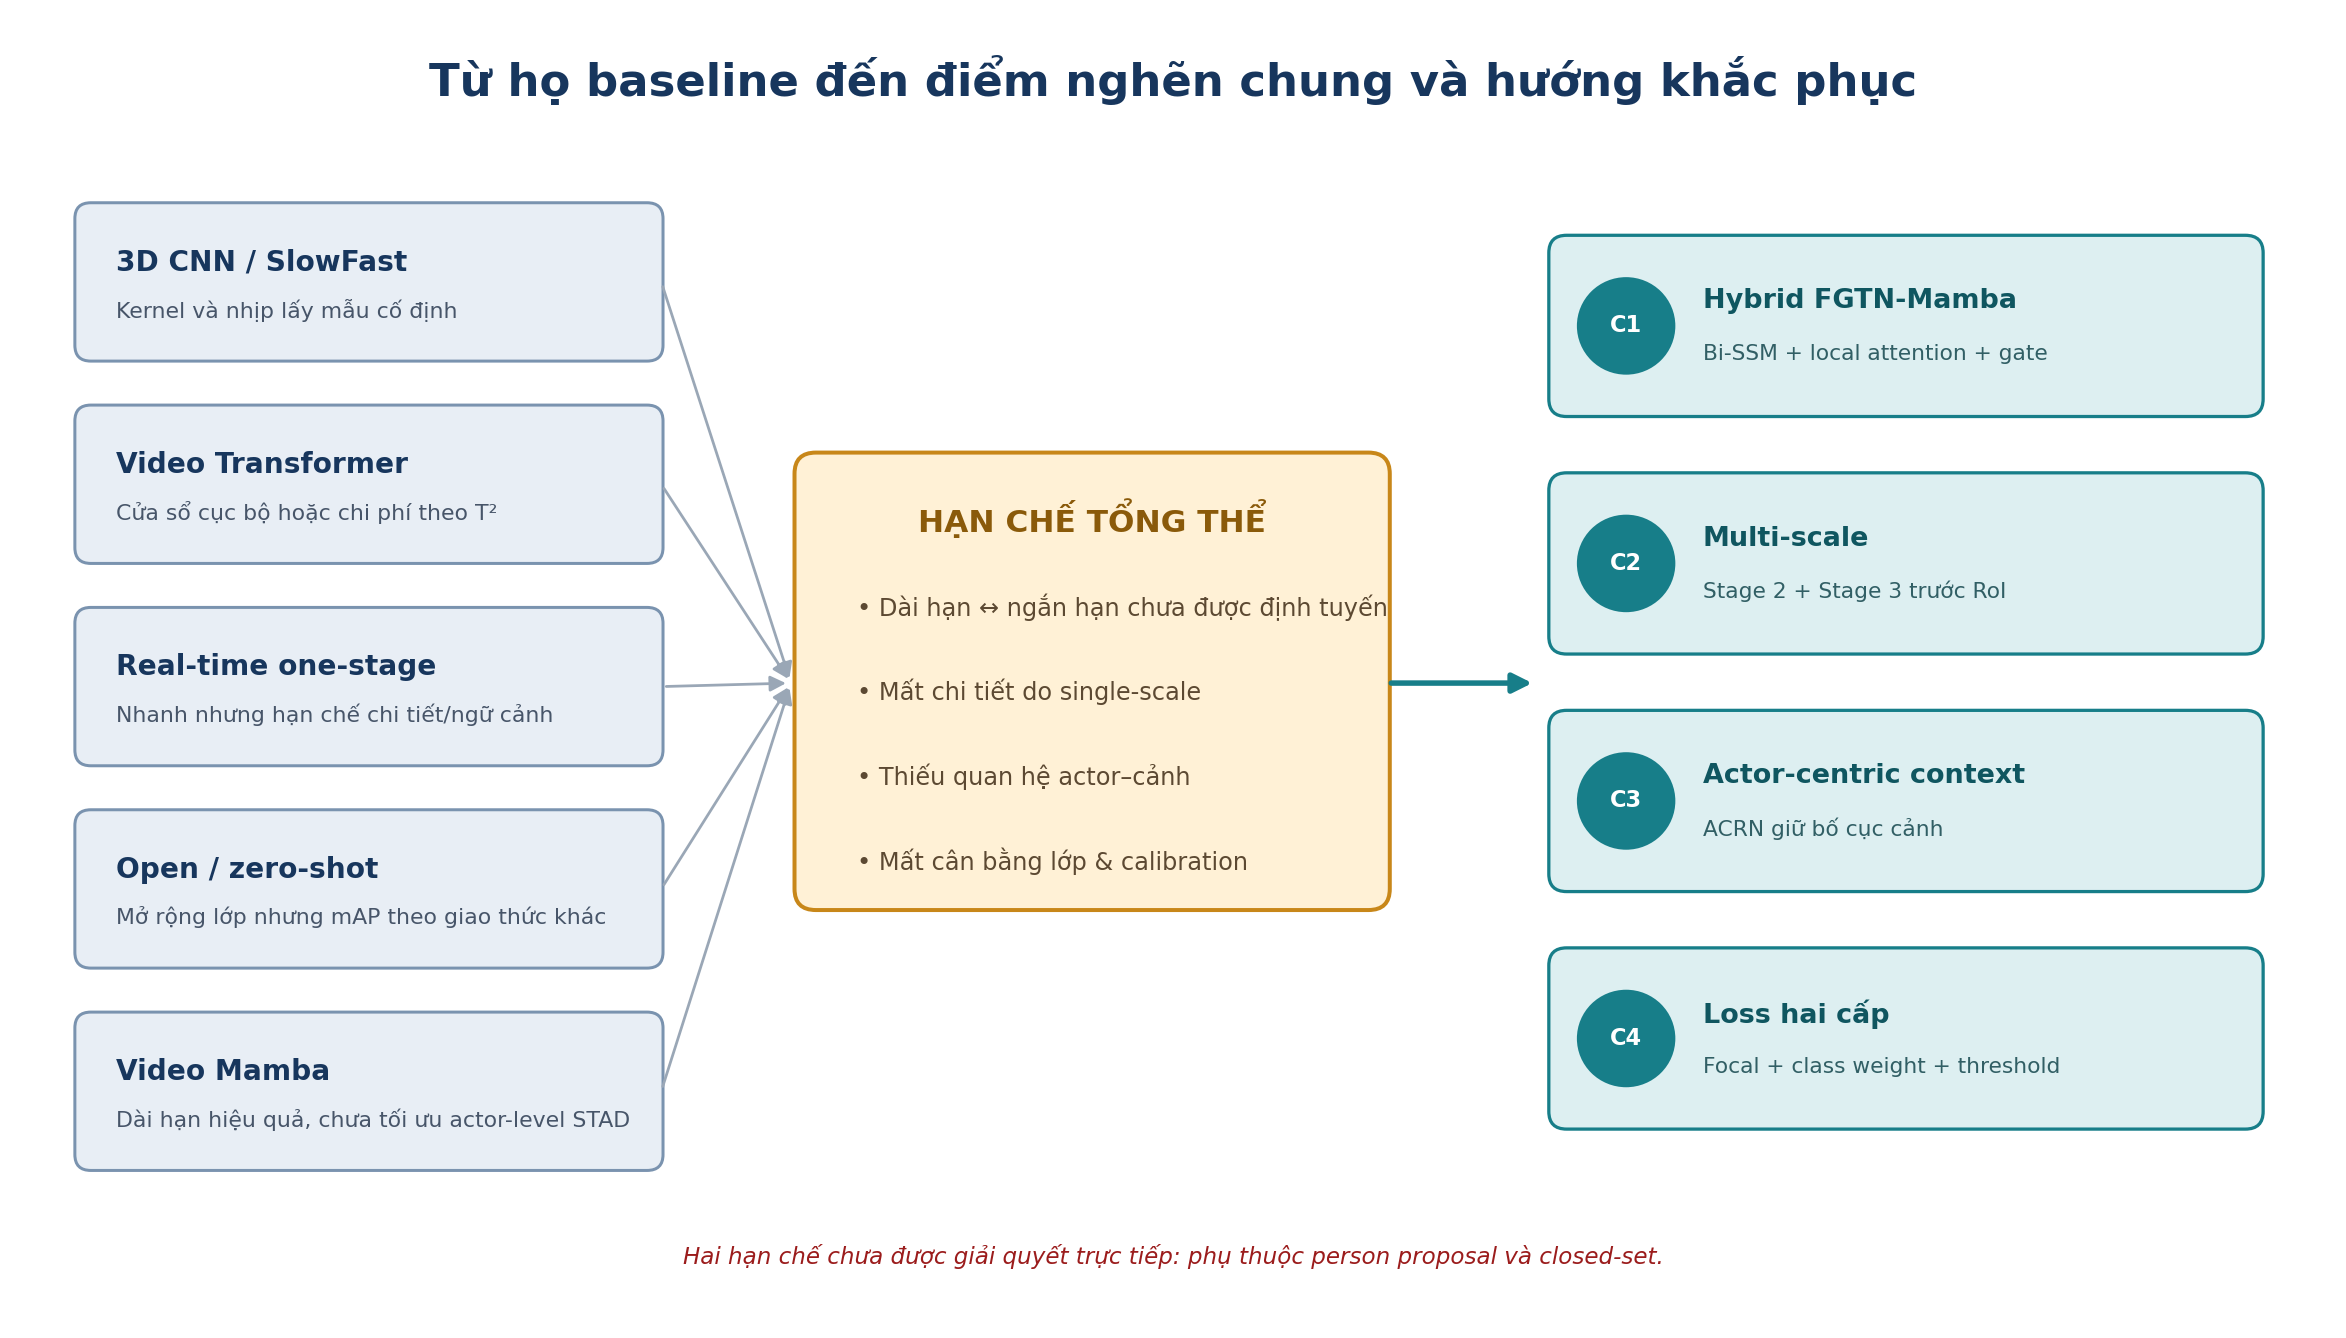
\includegraphics[width=\textwidth]{baseline_gaps.png}
\caption[Từ các họ phương pháp tới hạn chế chung và hướng khắc phục]{Từ các họ phương pháp tới hạn chế chung và bốn hướng khắc phục của luận văn: C1 --- Hybrid FGTN-Mamba (L1, L2); C2 --- đa tỉ lệ (L3); C3 --- ngữ cảnh lấy actor làm trung tâm bằng ACRN (L4); C4 --- hàm mất mát hai cấp và ngưỡng theo lớp (L5).}
\label{fig:gaps}
\end{figure}

\section*{Tiểu kết chương}
\addcontentsline{toc}{section}{Tiểu kết chương}

Chương này đã trình bày cơ sở lý thuyết của attention cửa sổ, mô hình không gian trạng thái chọn lọc, pipeline STAD hai giai đoạn và hàm mất mát cho dữ liệu mất cân bằng. Tổng quan bảy họ phương pháp cho thấy chưa có cơ chế nào vừa truyền ngữ cảnh dài hạn với chi phí tuyến tính, vừa giữ chuyển tiếp ngắn hạn và định tuyến giữa hai thang thời gian theo nội dung tại vị trí tiền-RoI của pipeline STAD theo từng người. Bảy hạn chế L1--L7 được ánh xạ tới các cơ chế xử lý trình bày trong \cref{ch:method}.
